

%/******************************************************************************
% *filename:		mokuaisheji.tex
% *author:  		synckey
% *version: 		v1.0
% *datetime:		2011-06-24 08:42:26
% *description:		模块设计
% *****************************************************************************/
\section{模块设计}
\subsection{线程池设计} 
在系统开始运行时创建MAXTHREAD个线程,放入线程池中。主线程创建监听套接字,开启服
务。每个线程各自调用accept,采用互斥锁来保证在每一个时刻只有一个线程调用accept。
每个线程在accept后为客户端服务。
\par{由于TCP内部为监听套接字维护两个队列:a.已完成队列,b.未
完成队列。所以在主线程睡眠期间,新的客户连接会使这两个队列充满(两个队列之和不超
过在listen时指定的backlog),而在这两个队列满了之后当一个客户的SYN到达时,TCP就
忽略该分节,也就时说,并不返回RST。这样做是因为:这种情况是暂时的,客户将重发SYN
,期望在不久就能在这些队列中找到可用空间\cite{unpv1}。 所以当这两个队列充满以后
,客户只是重发SYN ,而服务器不会接受客户端创建更多的连接。}
\begin{figure}[H]
\centering
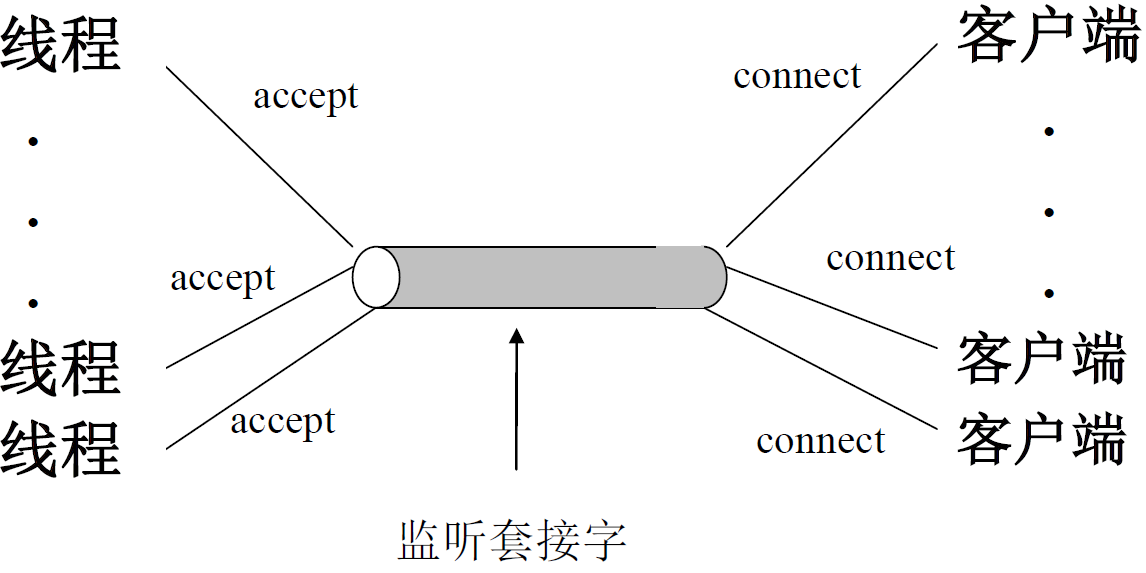
\includegraphics[keepaspectratio, scale=0.4]{pitures/xianchengmoxing.png}
\caption{多线程模型} 
\end{figure}
\subsection{工作线程设计}

线程池中的工作线程首先调用connect,接受一个客户端的连接,然后从报文的前4个字节中
获取报文的长度,从内存管理模块申请响应大小的内存,用于存放请求报文。
在收到请求后,逐次扫描每个域名。获得域名后,首先在本地的缓存中查找域名对应的IP,
如果有记录,就把IP地址填写到返回报文中,如果没有记录,则填入127.0.0.1,表明本地
没有缓存,将会进行DNS查询,结果在第二个报文中返回。然后把这个域名相应的序号和域
名填入到下图所示的链表中。

\begin{figure}[H]
\centering
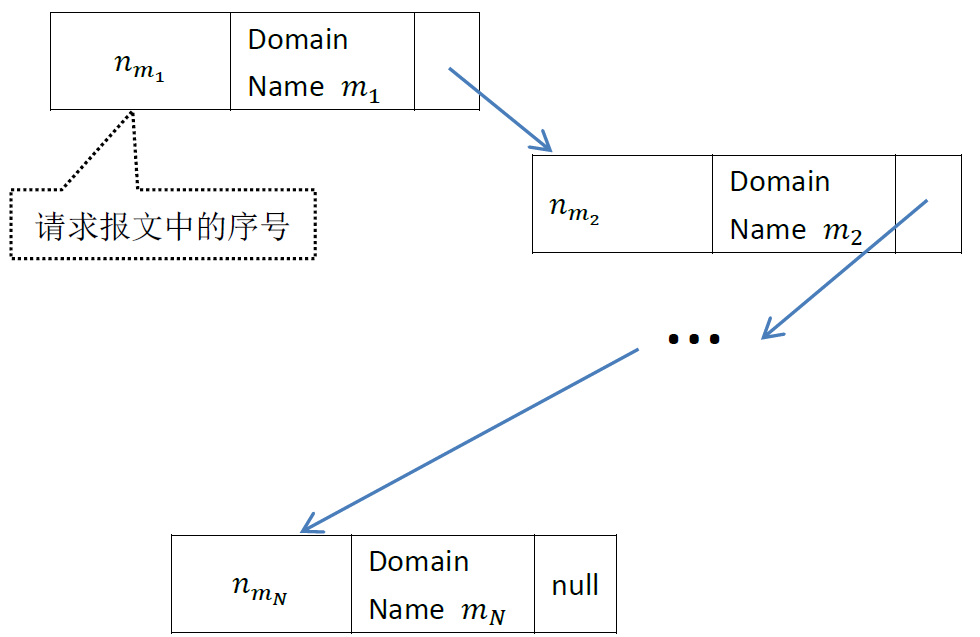
\includegraphics[keepaspectratio, scale=0.5]{pitures/response2_dns_list.png}
\caption{本地缓存未命中的域名构成的链表} 
\end{figure}

\par{工作线程在把请求报文遍历完毕后,就把第一次返回报文发送
给客户端,同时也把所有本地没有缓存的域名构造成了一个链表。如果链表为空,说明请求
的域名在本地都有缓存,任务完毕,关闭连接。否则,根据链表中的数目,申请用于构造第
二次返回报文的内存空间。对链表进行遍历,对链表中的每个域名调用一个DNS查询线程进行
DNS查询,在最后一个DNS查询完成后,把第二个报文发送给客户端,关闭连接。}

\begin{figure}[H]
\centering
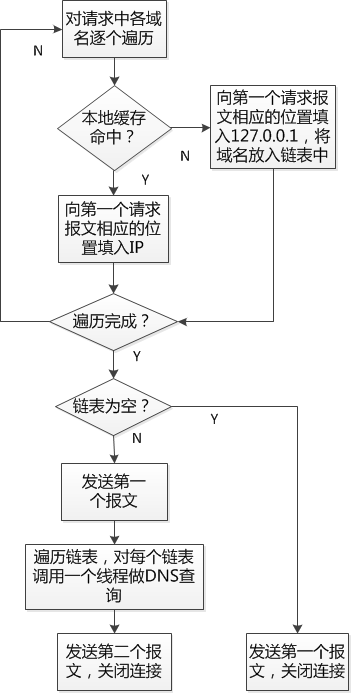
\includegraphics[keepaspectratio, scale=1]{pitures/xianchengliuchengtu.png}
\caption{线程工作流程图} 
\end{figure}


%%%%%%%%%%%%%%%%%%%%%%%%%%%%%%%%%%%%%%%%%%%%%%%%%
%                                               %
%filename	mm.tex				%
%author		wakemecn			%
%date		6/23/2011			%
%                                               %
%%%%%%%%%%%%%%%%%%%%%%%%%%%%%%%%%%%%%%%%%%%%%%%%%

%\documentclass{article}
%\usepackage{xeCJK}
%\setmainfont[BoldFont=SimHei]{SimSun%}
%\setmonofont{SimSun}
%\XeTeXlinebreaklocale"zh"
%\begin{document}
\subsection{内存管理模块}
		模块从系统预先申请256B,512B,1KB,2KB,$\ldots$,$2^n$KB等2幂次大小的块
		各若干。通过mem\_chunk结构维护特定大小的内存块大小的幂级,预分配的数目,
		已被使用的块链表和空闲的块链表。指针数组维护所有大小块的mem\_chuck结构
		指针。当申请使用M KB($2^m < M < 2^n$)空间时,若$2^n$KB大小块仍有空
		闲块,则将其分配,并将该块移动至已使用块链表中;若上述大小的块不存
		在空闲块或者不存在该大小的块,则模块动态申请若干数目该大小块的内存区域,
		分配内存。当释放某大小块时,若检测到释放的块位于模块动态申请的内存中
		时,则释放该内存。
\begin{figure}[H]
\centering
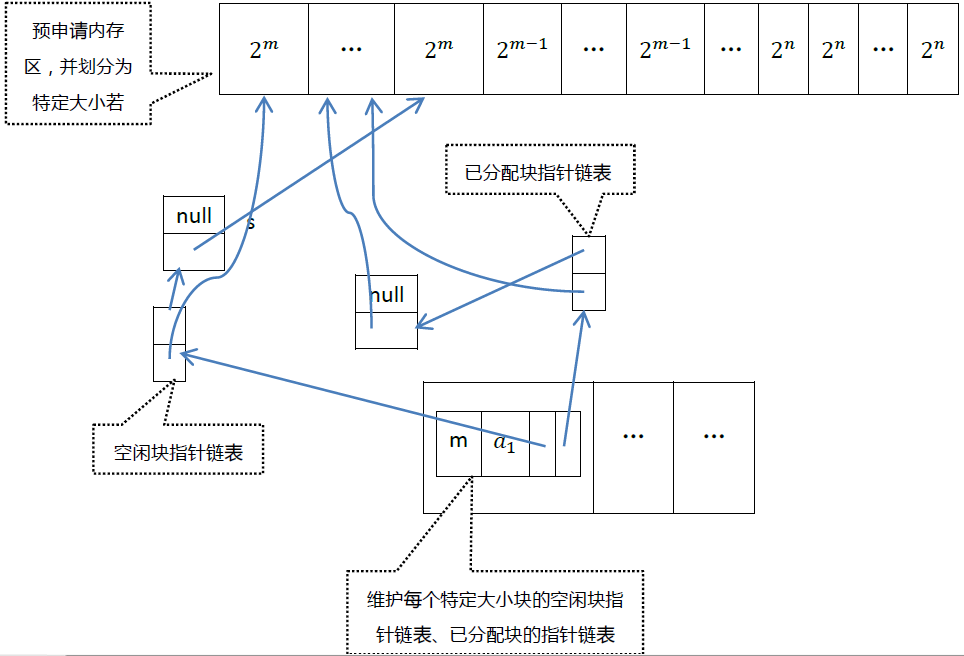
\includegraphics[keepaspectratio,scale=0.5]{pitures/mm.png}
\caption{内存管理示意图}
\end{figure}


%%%%%%%%%%%%%%%%	end of mm.tex    %%%%%%%%%%%%%%%


\subsection{缓存管理模块} 
\par{缓存管理模块由 DATrie 和 LIRS 栈驱动。}

\subsubsection{LIRS的定义}
\par{\textbf{DATrie:}双数组Trie(Double-Array  Trie,DATrie)是 trie 树的一个简单而有效的实现,
由两整数数组构成,一个是 base[],另一个是check[]。check[base[s] + c] = s base[s] + c = t。
}

\begin{figure}[H]
\centering
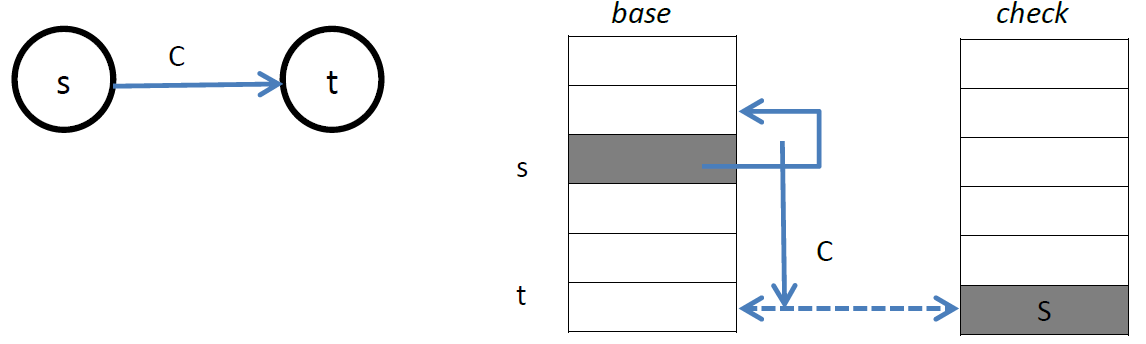
\includegraphics[keepaspectratio, scale=0.4]{pitures/aaa.png}
\caption{ DATrie 的状态转换示意,base[s]+c=t, check[t]=s } 
\end{figure}

\par{\textbf{LIRS:}最短最近使用间隔算法(Low  Inter-Reference  Recency  Set,LIRS):LIRS算法是一中基于LRU算法
	弱点而改进的算法,使用页面的最近实用间隔(Inter-Reference Recency,IRR)来决定要替
	换的页面。IRR用来表示一个页面的最近两次访问的间隔中的其他无重复页面的个数。
	LIRS还定义了最近访问时间R(Recency,R),用来表示一个页面的最近访问至当前访问之间
	的其它无重复页面的个数。
}

\begin{figure}[H]
\centering
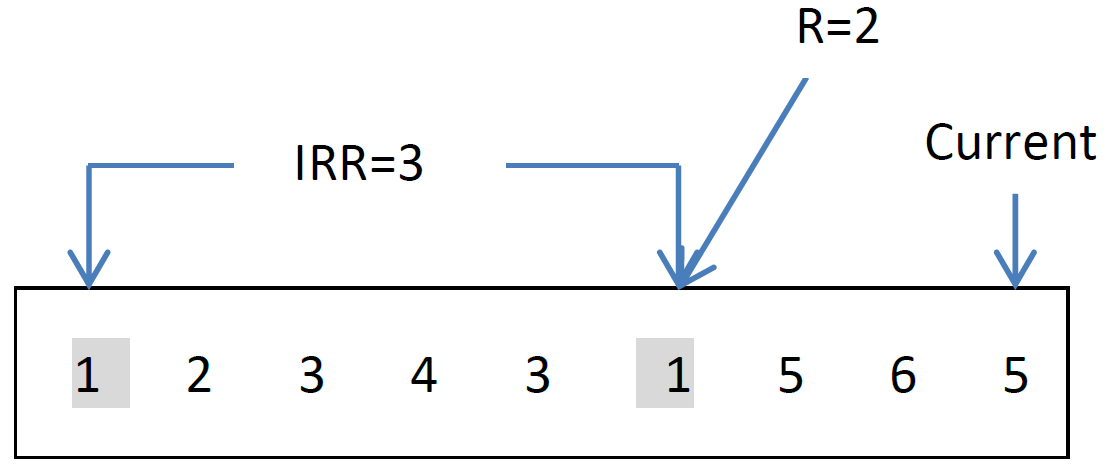
\includegraphics[keepaspectratio, scale=0.4]{pitures/irr.png}
\caption{LIRS算法的IRR和R的示意} 
\end{figure}

\subsubsection{DATrie的实现}
\par{	对域名集合的索引是由两个双数组字典(Double-Array Trie,DATrie)驱动的。其中
	一个 DATrie较大,存放所有已知域名集合,是静态的;另一个DATrie 较小,实际应用中作为较大的
	DATrie的补充,是动态变化的。每当动态DATrie 中记录达到一定数目时,就会离线补充静态DATrie
	中,失效域名从静态DATrie 中剔除。当有请求查询缓存是首先访问静态的DATrie,若没有命
中则访问动态DATrie,当两者均未命中时选择向动态 DATrie中插入记录。 
}

 静态DATrie 由离线生成,并且不断从动态 DATrie 中学习补充。 
\\ 域名索引不仅是对缓存内容索引,由于DATrie 查询字符串速度快,但插入或删除效率较低因此采用上
	述两个DATrie结合的缓存方法。 

\subsubsection{LIRS算法的实现}
LIRS算法的具体实现是由一个LIRS栈S和一个FIFO队列Q组成。
LIRS栈S维护LIR块,同时也维护常驻或非常驻状态的HIR块,FIFO队列Q维护所有常驻的HIR块。
\begin{figure}[H]
\centering
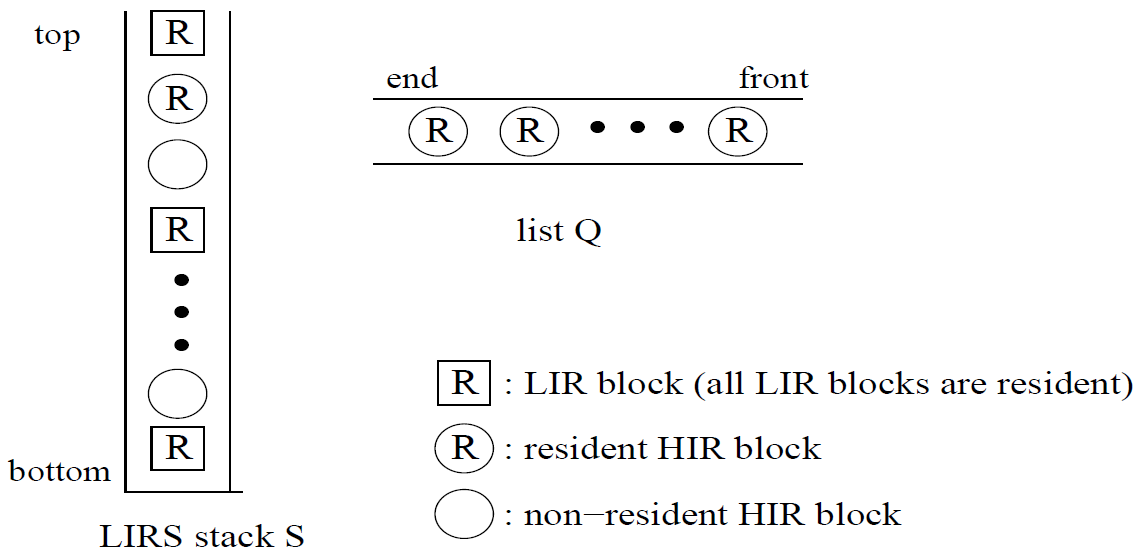
\includegraphics[keepaspectratio, scale=0.4]{pitures/lirsstack.png}
\caption{LIRS栈S维护LIR块,同时也维护常驻或非常驻状态的HIR块,FIFO队列Q维护所有常驻的HIR块。} 
\end{figure}


%/************`*********************  END OF mokuaisheji.tex  *********************************/
